\section{Broadcast Authentication & Device Pairing}

\subsection{Broadcast Authentication (Tesla)}

\paragraph{Broadcast Authentication:} 
\begin{itemize}
    \item One sender, a nr. of receivers (possibly malicious and unknown to the sender)
    \item All receivers need to verify the authenticity of the sender's messages
    \item We could do this with public-key crypto, but this is too expensive for some low power devices. 
\end{itemize}

\paragraph{Broadcast Authentication without PK Crypto:} Two approaches:
\begin{itemize}
    \item Delayed Key Disclosure (Cheung, Tesla)
    \item Presence Awareness
\end{itemize}

\subsubsection{Delayed Key Disclosure}
\begin{itemize}
    \item Uses purely symmetric primitives (MACs)
    \item Asymmetry from delayed key disclosure
    \item Self-authenticating keys (one-way hash chains)
    \item Requires loose time synchronization
\end{itemize}

\begin{minipage}{\linewidth}
    \centering      
    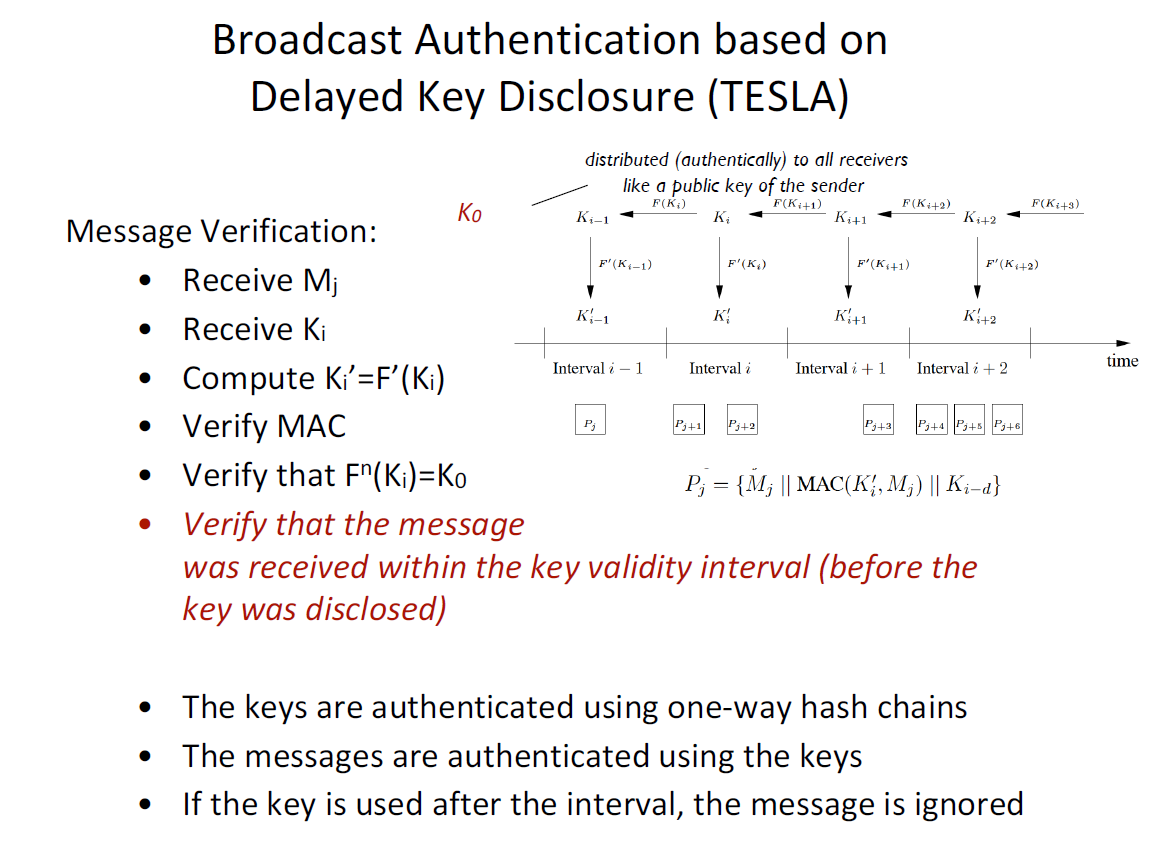
\includegraphics[width=\linewidth]{Figures/L8_tesla.PNG}
\end{minipage}

\subsection{Wireless Device Pairing}
\paragraph{Problem:} Given a pair of wireless devices without preloaded keys/credentials (mobile phones, printers), how do they establish a secret key in the presence of an adversary (passive or active (MITM attack))?

\subsubsection{Diffie-Hellman Protocol}
DH protocol enables secret key establishement by public communication. But DH is not secure against active attackers (MITM attaks). Therefore DH messages need to be authenticated, need PK crypto.

\subsubsection{Short String Comparison}
\begin{itemize}
    \item Establish key k using DH
    \item Hash the key h(k) and display on both devices
    \item Compare the displayed values (160 bits = 20 characters)
\end{itemize}

\subsubsection{Seeing is Believing}
Send the public key over an authentic channel (visual barcode / scanner)

\subsubsection{Loud and Clear}
Human-assisted string comparison using voice communication. A's PK transmitted over the wireless channel and h(pk) mapped to a reconizable sentence which i transmitted over wireless channel. B compares the the sentence to the hash of PK.

\subsubsection{Integrity Regions}
\begin{itemize}
    \item Establish key k using DH
    \item Authenticate DH keys by Physical proximity
    \item if the DH key comes from a close proximity it comes from a friend
\end{itemize}

\subsubsection{Shake Them Up}
\begin{itemize}
    \item Rely on the fact that the attacker does not know which device transmits at which time.
    \item Assume that A and B communicate over a wireless anonymous broadcast channel
    \item Eve can read the exchanged packets but cannot identify the src of the packets.
    \item Problems: Need synchronization (done through shaking), Signal fingerprinting (power, frequency,...)
\end{itemize}

\begin{minipage}{\linewidth}
    \centering      
    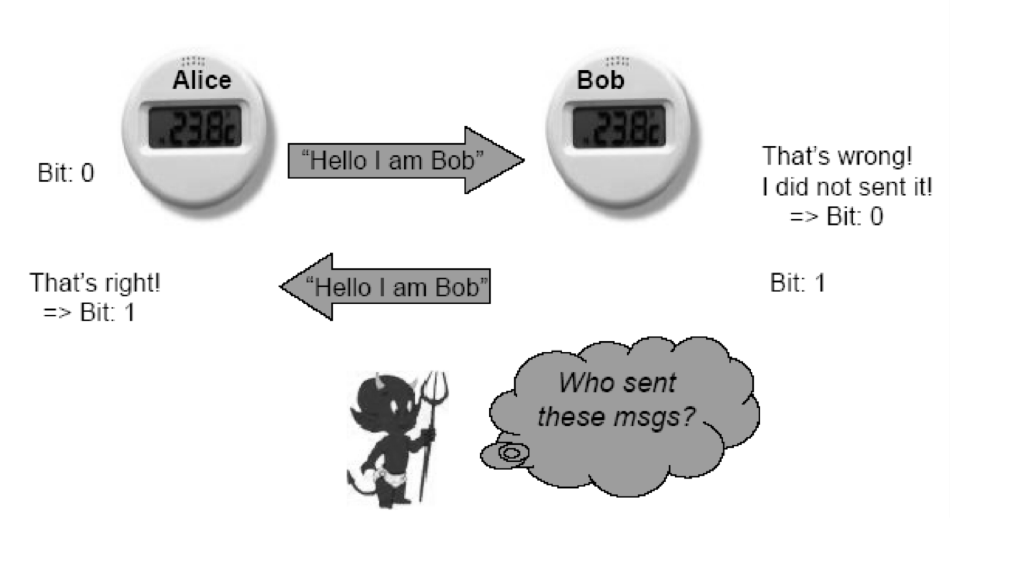
\includegraphics[width=\linewidth]{Figures/L8_shake_up.PNG}
\end{minipage}
